% Arch 4C --- Full LayerNorms + score-space private latent (M15c)
% Compile: tectonic arch4c_score_space.tex
\documentclass[11pt]{article}
\usepackage[a4paper,landscape,margin=14mm]{geometry}
\usepackage{lmodern}
\usepackage{amsmath,amssymb}
\usepackage{xcolor}
\usepackage{array,booktabs}
\usepackage{tikz}
\usetikzlibrary{arrows.meta,positioning,fit,backgrounds,calc}
\pagestyle{empty}
\setlength{\parindent}{0pt}
\newcolumntype{L}[1]{>{\raggedright\arraybackslash}p{#1}}

\definecolor{box}{HTML}{EEF2F7}
\definecolor{trn}{HTML}{FCE9C8}
\definecolor{frz}{HTML}{DCE6F2}
\definecolor{prv}{HTML}{E3F1DF}
\definecolor{nov}{HTML}{F8E6EF}

\tikzset{
  blk/.style={draw,rounded corners=3pt,fill=box,align=center,font=\normalsize,minimum height=18mm,text width=46mm,line width=0.8pt},
  frz/.style={blk,fill=frz},
  trn/.style={blk,fill=trn},
  prv/.style={blk,fill=prv},
  nov/.style={blk,fill=nov},
  lab/.style={font=\footnotesize,text=black!80,inner sep=1.5pt},
  ar/.style={-{Latex[length=3mm]},line width=1.1pt}}

\begin{document}

\begin{center}
{\Large\bfseries Arch 4C --- Full LayerNorms + Score-Space Private Latent (M15c)}\\[2pt]
{\small Keeps Arch~1's LN capacity (protects NT) but replaces GBLA LN-offsets and the linear head. Private latent is tiny and lives in \textbf{score / margin space}.}
\end{center}
\vspace{3mm}

\begin{center}
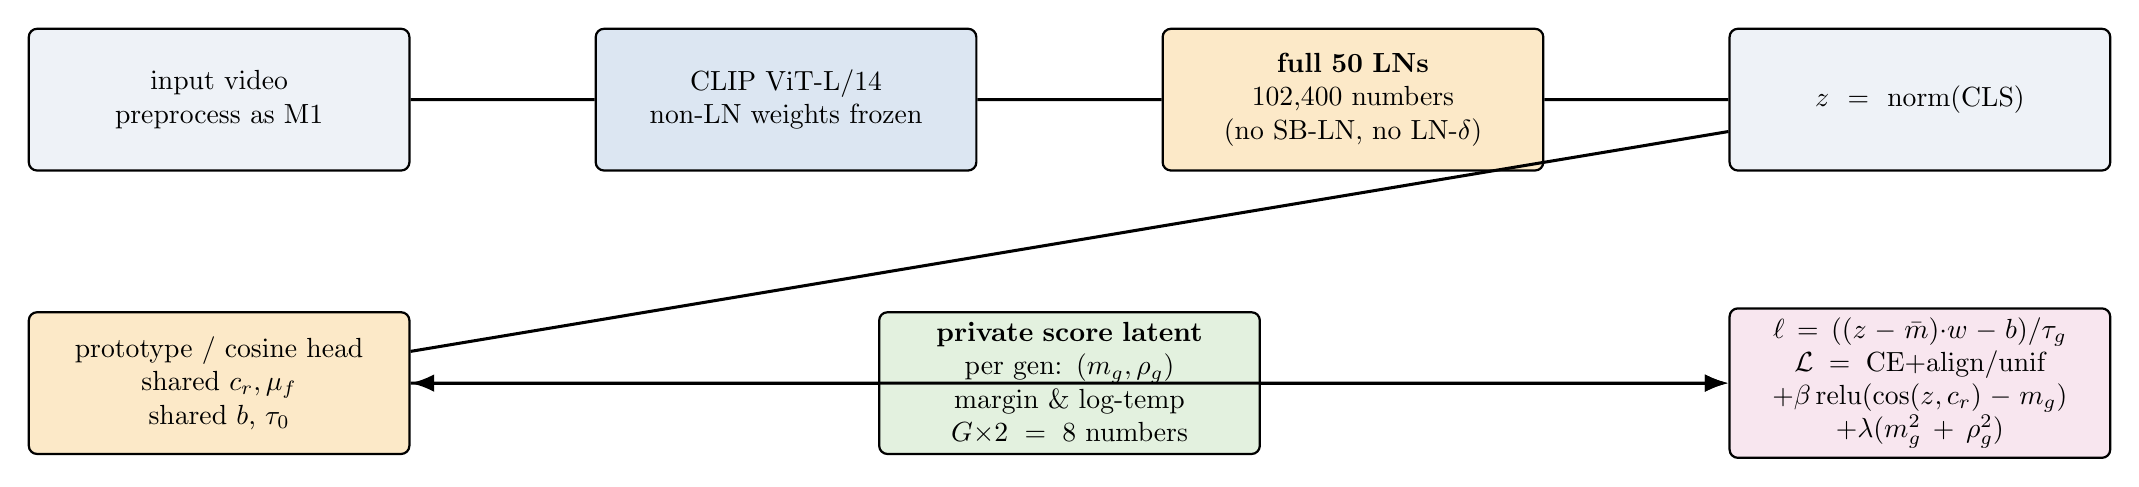
\begin{tikzpicture}[x=72mm,y=-36mm]
\node[blk] (vid) at (0,0) {input video\\preprocess as M1};
\node[frz] (enc) at (1,0) {CLIP ViT-L/14\\non-LN weights frozen};
\node[trn] (ln) at (2,0) {\textbf{full 50 LNs}\\102{,}400 numbers\\(no SB-LN, no LN-$\delta$)};
\node[blk] (z) at (3,0) {$z=\mathrm{norm}(\mathrm{CLS})$};
\node[trn] (proto) at (0,1) {prototype / cosine head\\shared $c_r,\mu_f$\\shared $b$, $\tau_0$};
\node[prv] (sc) at (1.5,1) {\textbf{private score latent}\\per gen: $(m_g,\rho_g)$\\margin \& log-temp\\$G{\times}2=8$ numbers};
\node[nov] (loss) at (3,1) {$\ell=((z-\bar m){\cdot}w-b)/\tau_g$\\$\mathcal{L}=\mathrm{CE}+$align/unif\\$+\beta\,\mathrm{relu}(\cos(z,c_r)-m_g)$\\$+\lambda(m_g^2+\rho_g^2)$};
\draw[ar] (vid)--(enc)--(ln)--(z)--(proto)--(loss);
\draw[ar] (sc)--(loss); \draw[ar] (sc)--(proto);
\end{tikzpicture}
\end{center}

\vspace{4mm}
\begin{center}
{\normalsize\bfseries Why this is not Arch 1 / 2 / 3}
\end{center}
\vspace{2mm}
\begin{center}
\small
\begin{tabular}{L{35mm}L{50mm}L{50mm}L{50mm}}
\toprule
 & Arch 1 & Arch 3 & \textbf{Arch 4C} \\
\midrule
LN path & full + LN-$\delta$ & SB-LN + feat-$\delta$ & full LN, \textbf{no} LN-$\delta$ \\
head & linear 2{,}050 & prototype & prototype \\
private & $\delta$ on $\gamma,\beta$ & $W\delta$ on $\mu_f$ & $(m_g,\rho_g)$ on \textbf{scores} \\
loss link & $\lambda\|\delta\|^2$ & PFAL to $c_f(\delta)$ & margin/temp in CE+margin loss \\
deployed $P$ & 104{,}450 & 34{,}370 & $\approx$102{,}402 \\
\bottomrule
\end{tabular}
\end{center}

\vspace{5mm}
\begin{center}
\small
\begin{tabular}{L{60mm}rr}
\toprule
piece & count & deployed? \\
\midrule
full LayerNorms & 102{,}400 & yes \\
prototype $b,\rho_{\mathrm{shared}}$ & 2 & yes \\
private $(m_g,\rho_g)$ & 8 & \textbf{no} \\
\textbf{deployed} & 102{,}402 & $<104{,}450$ \\
\bottomrule
\end{tabular}
\hspace{8mm}
\begin{tabular}{L{55mm}L{70mm}}
\toprule
aim & met by \\
\midrule
1 & prototype head; no linear; no GBLA offsets \\
2 & margin/temp-conditioned loss \\
3 & $(m_g,\rho_g)$ inside CE + relu margin + $\lambda$ \\
4 & 102{,}402 $<$ 104{,}450 (drops linear 2{,}050) \\
\bottomrule
\end{tabular}
\end{center}

\vfill
{\small Notebook: \texttt{M15c.ipynb}. Highest chance to hold NT (full LNs) while still claiming a new head/loss/private link distinct from published GBLA. Decision: KEEP iff NT $\ge$ A0 and DFD $\ge95.5$ (same pre-registered honesty).}

\end{document}
